\documentclass{scrartcl}

\usepackage[utf8]{inputenc}
\usepackage[T1]{fontenc}
\usepackage{lmodern}
\usepackage[ngerman]{babel}
\usepackage{amsmath}
\usepackage{listings}
\usepackage{graphicx}
\usepackage{float}

\usepackage{color}

%% Commands
\newcommand{\n}{\newline}

\title{Diary}
\subtitle{King of Jawa}
\author{Isabel Geissmann, Jannik Jaberg}
\date{Stand \today}
\begin{document}

\maketitle
\begin{figure}[H]
	
\includegraphics[width=\linewidth]{LOGO.png}
\end{figure}


\section*{Eintrag vom 11. April 2018}
Folgende Punkte zum Meilenstein 3 haben wir bereits fertiggestellt:
\begin{itemize}
	\item Broadcast \n
	\item Commandline \n
	\item Chat GUI \n
	\item GameState ist auf dem Server \n
	\item Playerlist \n
	\item Gamelist \n
	\item Whisper \n	
\end{itemize}	
Folgende Punkte müssen wir noch abarbeiten:

\begin{itemize}
	\item  Protokoll muss aktualisiert werden\n
	Isabel HighscorePackge\n
	Jannik LobbyPackage
	\item Highscore \n
	Der Highscore funktioniert nur wenn das Spiel über die Commandline gestartet wird. Wird das Spiel mit der Jar-Datei gestartet funktioniert das Auslesen der txt-Datei nicht. 
	\item Game ist spielbar \n
	Gebäude können auf der Karte gesetzt werden aber die GameLogic muss noch verknüpft werden. 
	\item QA \n
	Pascal hat das QA mit Marco angeschaut und wir werden noch hinzufügen, dass die Methoden nicht länger als eine gewisse Anzahl von Zeilen sein soll. 
	\item Library \n
	Log4J muss noch eingebunden werden. 
	\item Lobby \n
	Lobby muss gestartet werden können:\n
	Button Create Lobby $\rightarrow$ neues Fenster, Map auswählen und Lobby erstellen oder gestartete Lobby im Hauptmenu auswählen und joinen.
	
\end{itemize}

\section*{Eintrag vom 10. April 2018}
Heute arbeiten wir gemeinsam am Programmierprojekt weiter. Zu Beginn erklärt uns Pascal die Umstrukturierung der Projektstruktur und die Änderungen die er im Kommunikationsprotokoll vorgenommen hat. Die Priorität haben wie nach dem Feedback von Meilenstein 2 herausgelöscht und einige Verbesserungen vorgenommen. 

\begin{itemize}
	\item Package Types \n
	Sind in einer Enum Klasse definiert.
	\item Package \n
	Jades Package hat seine eigene Klasse:
	\begin{itemize}
		\item ChatPackage, ConnectionPackage, PingPackage, UserPackage
		\item Heute werden folgende Package hinzugefügt:
		\begin{itemize}
			\item HighscorePackage (Isabel)
			\item LobbyPackage (Jannik)
		\end{itemize}
	\end{itemize}
	\item Handler\/Manager \n
	Jedes Package hat Server- bzw. Client-Seitig einen Handler und einen Manager. 
\end{itemize}
Wir haben in einigen Branches gleichzeitig gearbeitet. Nikolai und Pascal mergen alle Branches auf den Masterbranch und verknüpfen die verschiedenen Schnittstellen miteinander als Vorbereitung auf den Meilenstein 3.
%% MapRendering
\section*{Eintrag zum MapRendering}
Ein Anspruch von uns an unser Spiel ist, dass es nicht nur 2D dargestellt wird, sondern in einem fake 3D bzw. in einer isometrischen Ansicht. Jannik hat sich innig damit beschäftigt und einen Prototypen in Swing erstellt. Siehe Abbildung \ref{fig:map1}\n
In einem zweidimensionalen Array wird jedes einzelne Quadrate (Tiles) umgerechnet. Für die Umrechnung haben wir die Methoden toIso() und toCartesian() geschrieben. Beim ersten Rendern der Map dauert es etwas länger da jedes Tile einzeln ausgerechnet werden muss. Als der Prototyp fertiggestellt war, haben wir uns Gedanken darüber gemacht wie wir die Struktur in unserem Spiel aufbauen wollen. \n
\n
Unsere Idee:\n
Die Map wird auf dem Server und auf dem Client geladen. Auf dem Client muss die Map im Userinterface angezeigt werden. Auf dem Server benötigen wir nur die Tile Repräsentation damit wir die Tiles mit unserer Spiellogik verknüpfen können. Wenn ein Spieler etwas bauen will wird beim Server angefragt ob dies erlaubt ist oder nicht. Falls gebaut werden darf, wird das Gebäude auf dem Server gebaut und an alle Clients gesendet.


%%BILD
\begin{figure}[H]
	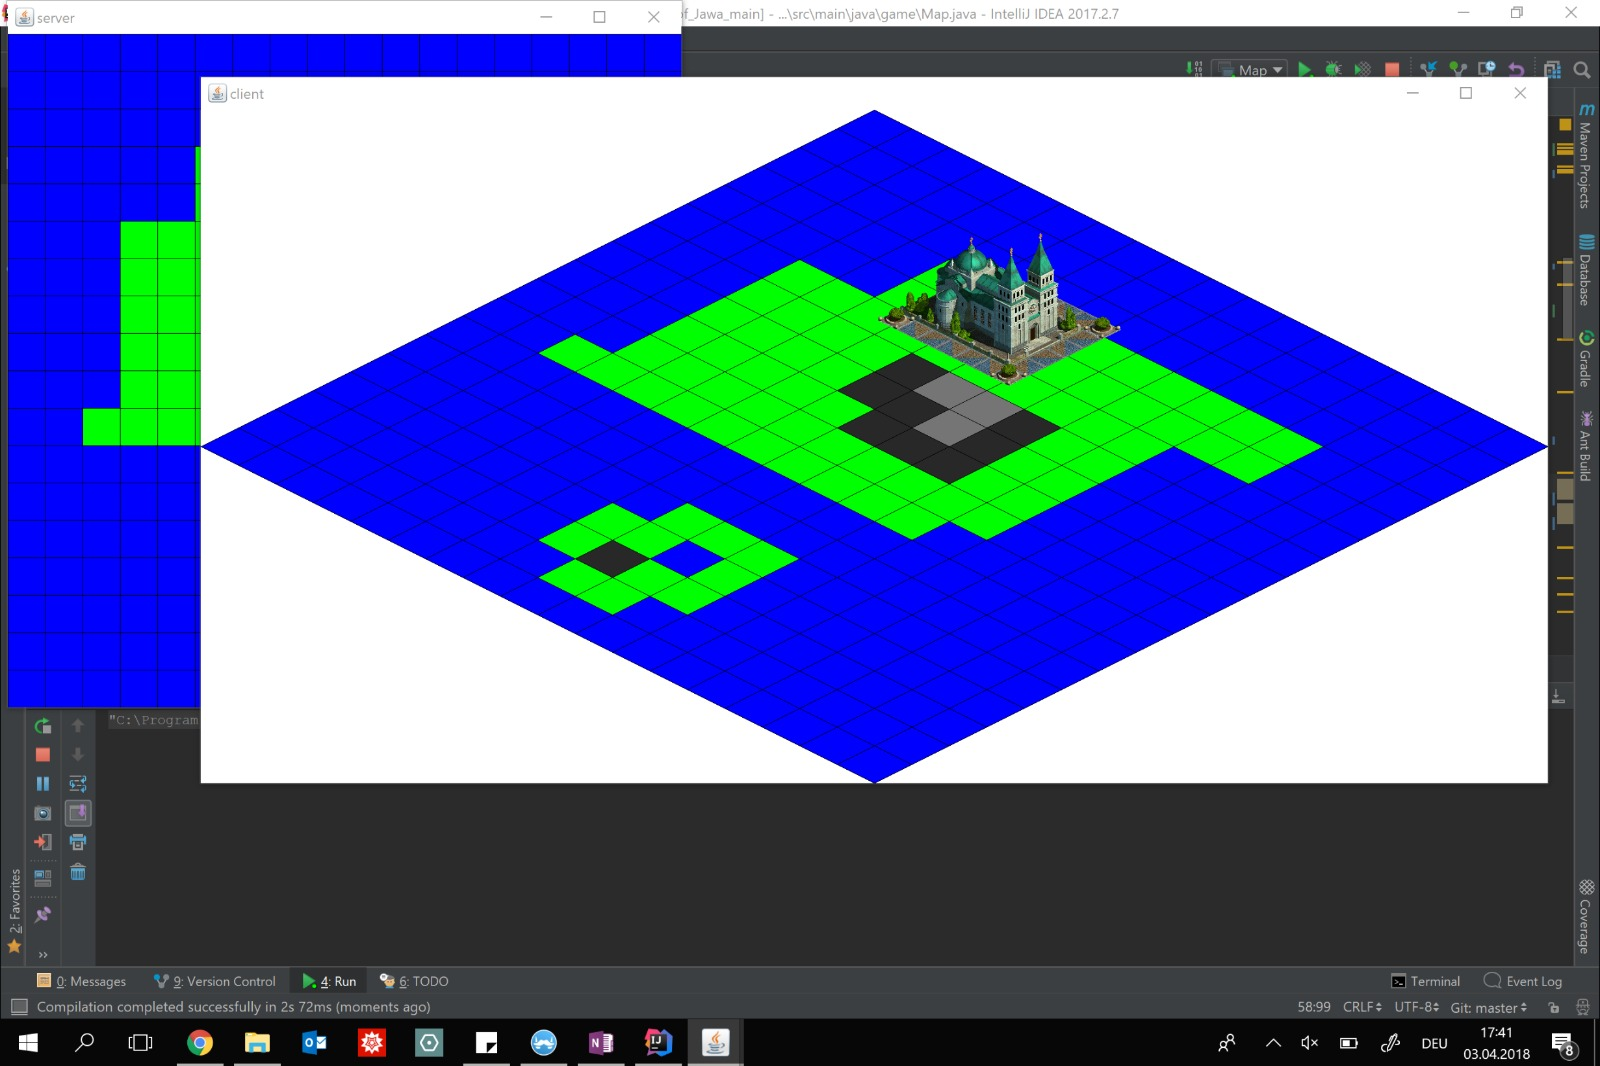
\includegraphics[width=\linewidth]{map1.jpeg}
	\caption{Testlauf der Map.}
	\label{fig:map1}
\end{figure}
Alle Berechnungen und die gesamte Spiellogik spielen sich auf der "Kartesischen Karte" ab und nur der Teilausschnitt der beim Spieler angezeigt wird, wird ins "isometrische Kartensystem" umgerechnet und im Userinterface angezeigt. Sonst hätten wir pro Sekunde 1 Billion Operation um die gesamte Map für jeden Spieler zu aktualisieren. \n
Im JavaFX haben wir zwei Canvas Elemente die gleich gross sind, zum einen die Game Canvas und die Heads-Up-Display Canvas. Wenn auf dem HUD Canvas kein Element verfügbar ist auf das geklickt werden kann wird man automatisch an das Game Canvas weitergeleitet. Im Game Canvas ist die gesamte Map gespeichert und auf dem HUD Canvas haben wir verschieden Elemente wie zum Beispiel die Minimap. 

\section*{About the Game}
Hauptziel: Aufbau einer Zivilisation mit Metropolenstatus.\n
Das Spiel ist in drei Phasen aufgeteilt:
\begin{itemize}
	\item Insel aussuchen und Basis bauen
	\item Bau von Ressourcengebäuden (Minen, Farmen, etc.) um damit die entsprechenden Ressourcen zu sammeln
	\item Verbesserungen der Gebäude (Aufstieg in höhere Level) damit schneller Ressourcen gesammelt werden können
\end{itemize}
\begin{figure}[H]
	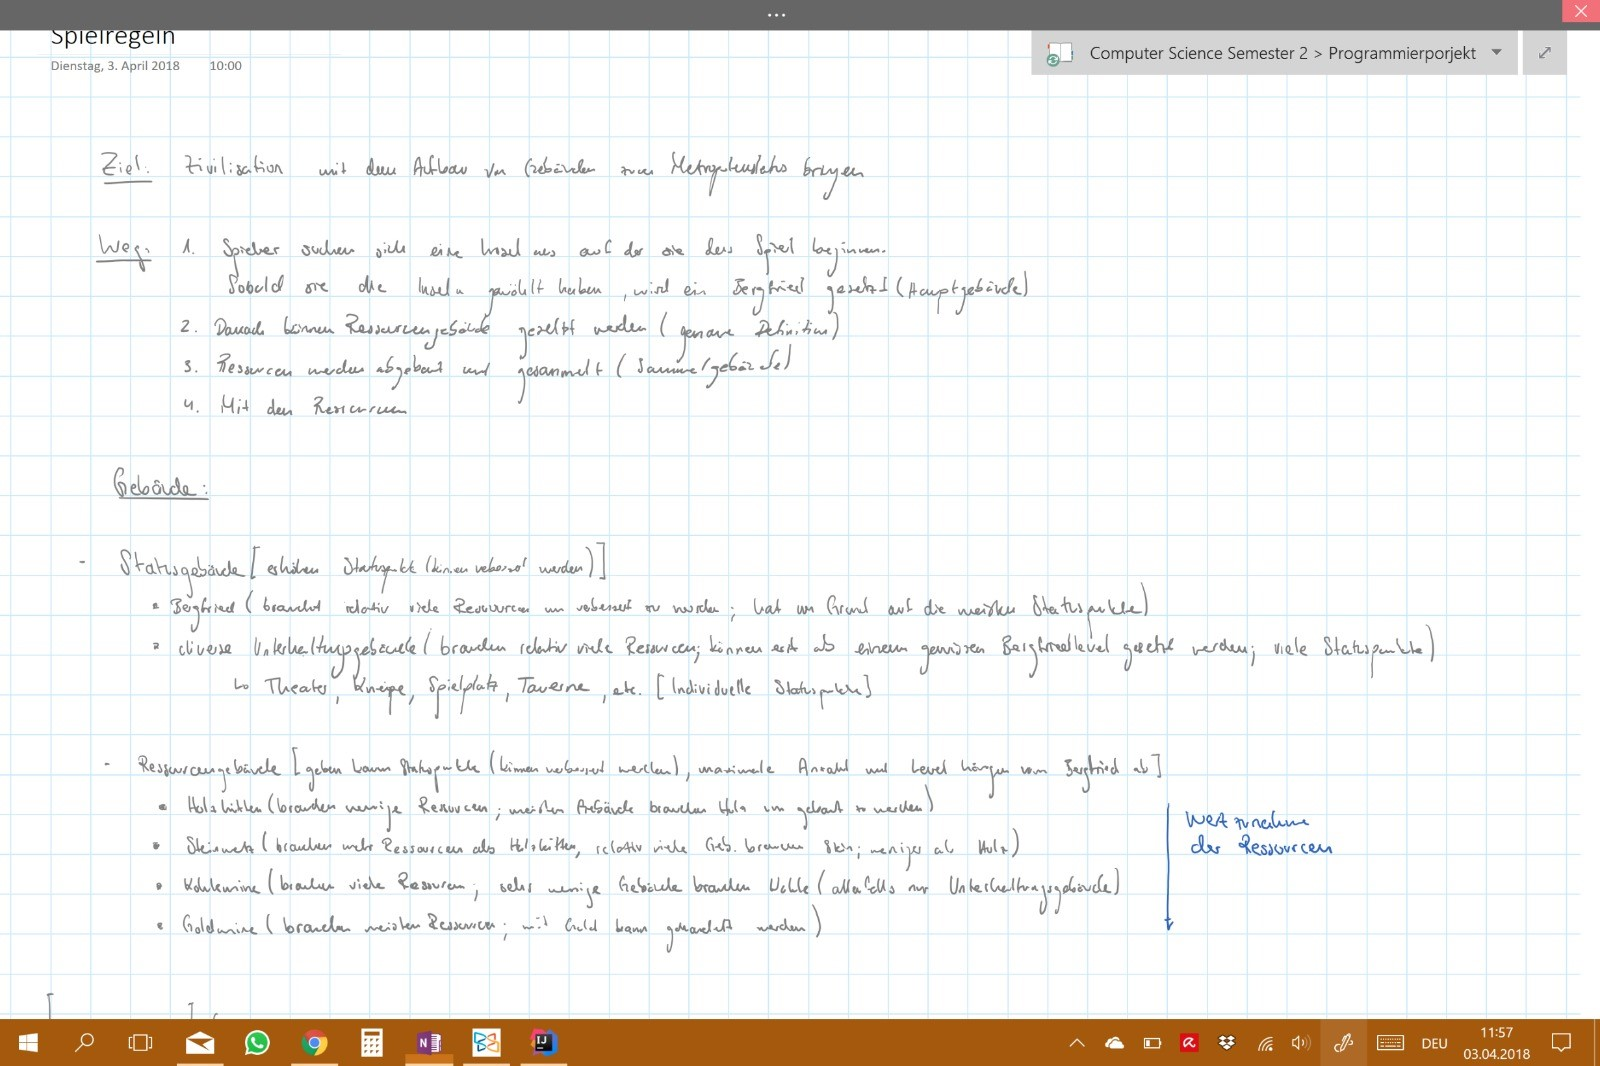
\includegraphics[width=\linewidth]{Idee1.jpg}
	\caption{Erste Ideen von Nikolai 1}
	\label{fig:map1}
\end{figure}
Aus der Diskussion was wir für den dritten Meilenstein zur basic GameLogic alles benötigen, hat sich folgendes ergeben. Es muss möglich sein eine Insel auszuwählen und eine Basis zu bauen. Sobald die Basis gebaut ist kann das erste Ressourcen-Gebäude gebaut werden. Um Steuern einzunehmen muss auch gleich das erste Einfamilienhaus gebaut werden.\n
Um die basic GameLogic zu zeigen benötigen wir daher nur ein Ressourcen-Gebäude, mit dem wir eine Ressource (z.B. Holz oder Stein) generieren können und Bewohner die Steuern bezahlen. Dies ist die Basis für das gesamte Spiel. \n
Zu einem späteren Zeitpunkt werden noch weitere Gebäudearten hinzugefügt. Dann können wir auch noch genau festlegen, wie wir die verschiedenen Level der Gebäude bzw. der Basis festlegen möchten. \n\n
Das Spiel kann beliebig erweitert werden, zum Beispiel:
\begin{itemize}
	\item Ressourcengebäude: \n
	Supermärkte, Steinmetze, Goldminen, Eisen, Kohle, Kaffee, Diamanten, Wolle
	\item Spassgebäude: \n
	Theater, Taverne, Bordell, Thermen
	\item Bildungsbebäude: \n
	Uni Basel, Kirche, Mosche, Tempel, Opfergebäude, Altar
	\item Verwaltungsgebäude: \n
	Gericht, Gefängnis, Verwaltung
\end{itemize}

\begin{figure}[H]
	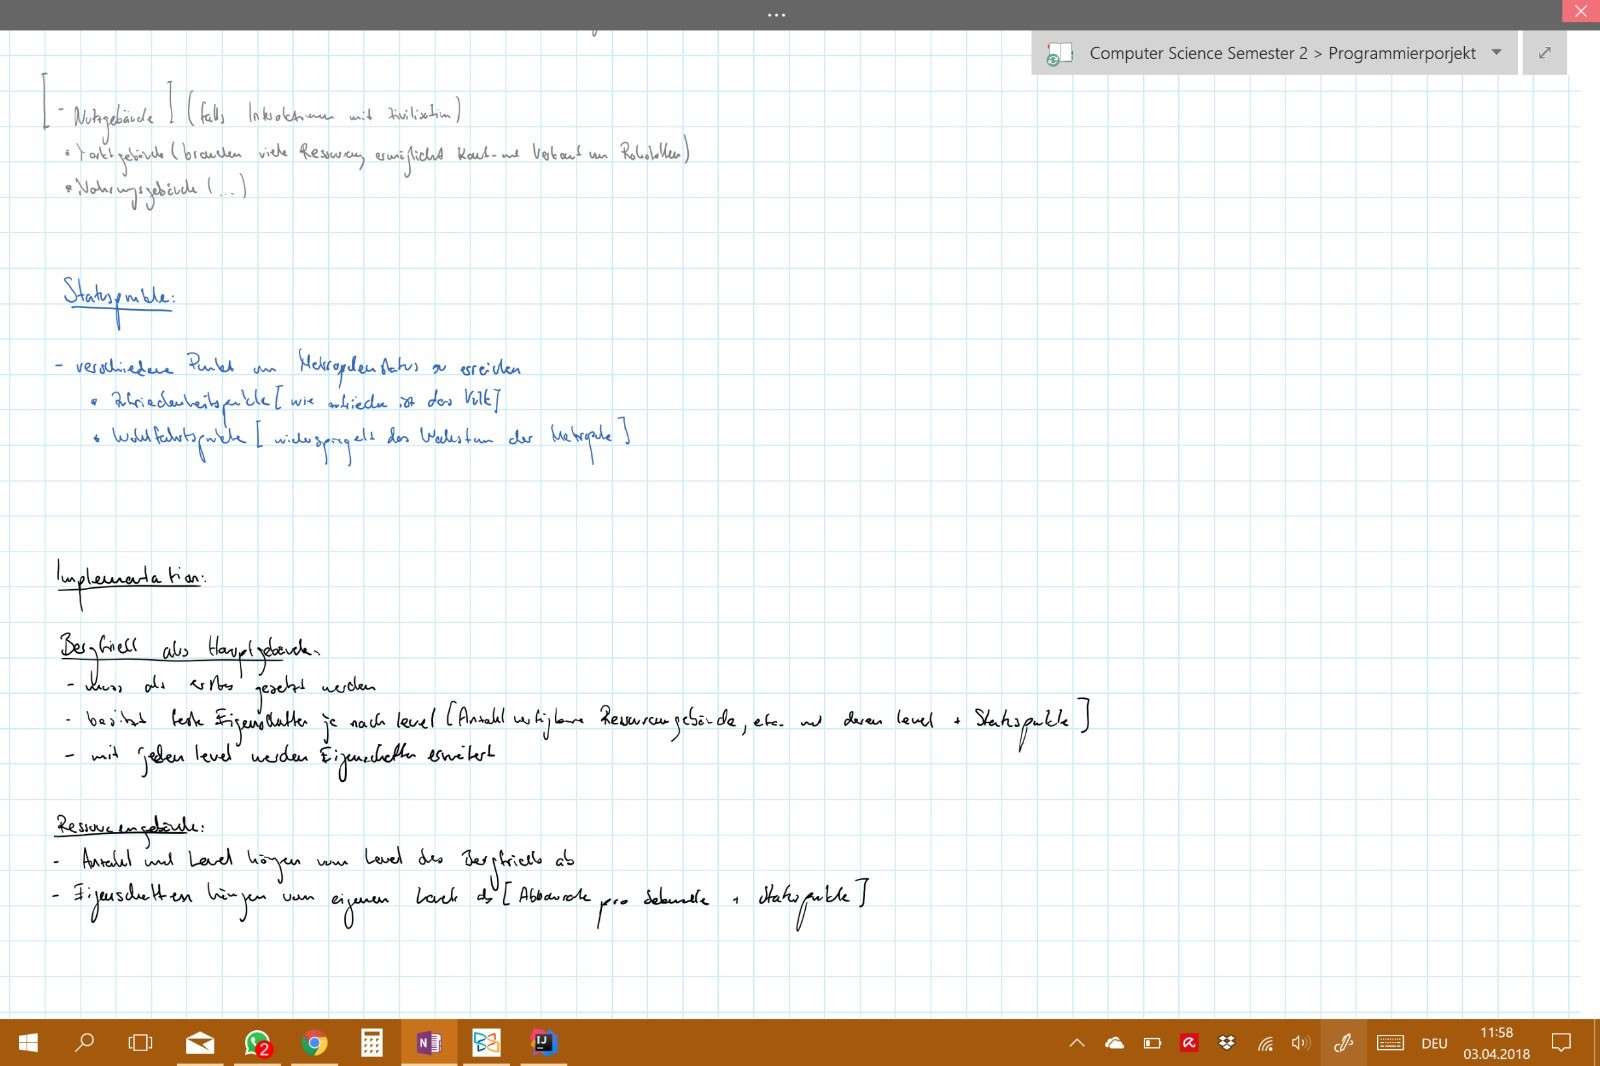
\includegraphics[width=\linewidth]{Idee2.jpg}
	\caption{Erste Ideen von Nikolai 2}
	\label{fig:map1}
\end{figure}



\section*{Eintrag vom 3. April 2018}
Bevor am Programmierprojekt weiter gearbeitet haben sind wir die Punkte für den Meilenstein 3 durchgegangen und haben alles besprochen. \n
\begin{itemize}
	\item About the Game\n
	Wir hatten bereits eine sehr gute Grundidee, diese wird nun von Nikolai ausgearbeitet und in diesem Diary Eintrag angehängt. Sobald die Ideen ausgearbeitet sind werden wir diese Ideen gemeinsam durchgehen und besprechen. 
	\item Broadcast \n
	Jannik wird bei Marco nachfragen wie dieser Punkt zu verstehen ist. Sobald er eine Antwort erhält wird er alle updaten.
	\item Build Script \n
	Die ausführbare Jar-Datei ist bereits funktionsfähig. Im nächsten Schritt werden wir das Erstellen des Java Docs im Gradle einbinden, damit dies automatisiert wird.
	\item Commandline \n
	Jannik wird den Code anpasse, dass das Starten des Spiels mit den vorgegebenen Parametern funktioniert.\n
	$(client <hostadress>:<port> [<username>]  |  server <port>)$
	\item Chat im GUI \n
	Isabel hat bereits einen Entwurf des Userinterface für den Chat erstellt. Heute werden Pascal und Isabel das Userinterface mit dem Code verknüpfen.
	\item Gamelist \n
	Im Userinterface soll eine Liste mit allen Lobbies erstellt werden. Bei jeder Lobbie wird der aktuelle Status waiting, running, paused oder finished angezeigt. Die Eigenschaften einer Enum Klasse kommen uns hier sehr entgegen, da wir nur diese 4 verschiedenen Status verwenden wollen. 
	\item GameLogic \n
	Für diesen Meilenstein soll die Game Logic in einer einfachen Form bereits implementiert und spielbar sein. Damit wir unsere Game Logic im Spiel umsetzten können müssen wir zuerst das Rendering der Map und das Entity System fertigstellen. Um die Umsetzung der Game Logic kümmern wir uns in der Kalenderwoche 15.
	\item GameState \n
	Der Server leitet alles an den Client weiter, es sollen keine Daten die das Spielgeschehen beeinflussen auf dem Client sein, damit der Client nicht cheaten kann. 
	\item Highscore \n
	Im Userinterface soll der Highscore angezeigt werden. Der Highscore muss in einem File gespeichert werden, damit dieser auch nach einem Neustart des Spiels noch sichtbar ist. Im Highscore soll der Spielname, der Gewinner, die zu erreichende Punktzahl und die benötigte Zeit angezeigt werden. So haben wir später die Möglichkeit verschiedene Spielmodi zu implementieren. Zum Beispiel eine Speed Runde in der nur 200 Punkte für den Metropolenstatus benötigt werden.
	\item Library \n
	Pascal wird nachfragen ob JavaFX als Library gezahlt wird. Falls JavaFX keine Library ist werden wir Log4J in unserem Spiel hinzufügen. Damit Error Logs schön angezeigt und gespeichert werden können. Dies vereinfacht und das Debugging. \n
	$\rightarrow$ JavaFx zählt nicht als Library.
	\item Manual \n
	Das Manual werden wir erst weiterschreiben sobald unser Userinterface und die Game Logic fertig sind. Damit wir diese nicht ständig anpassen müssen. 
	\item Playerlist \n
	Im Userinterface soll eine Liste der Spieler die online sind angezeigt werden. Sobald ein Spieler seinen Namen ändert muss dieser auch in der Spielerliste geändert werden. Sollten wir noch genügend Zeit haben möchten wir noch einen Rechtsklick hinzufügen um eine Direktnachricht an den jeweiligen User zu senden. 
	\item Protocol \n
	Alle neuen Packages müssen im Protokoll fortlaufend dokumentiert werden. 
	

\end{itemize}

\section*{Milestone 2}
Wir haben den zweiten Meilensteil erfolgreich gemeistert und unsere Ziele grösstenteils erreicht. Für den nächsten Meilenstein haben wir einige Dinge, die wir anders handhaben müssen. Alle Tagebucheinträge werden zusätzlich zur Webseite auch in einem PDF gespeichert und auf den master branch gepusht. In unserem Protokoll werden wir die Priority löschen. Wir benötigen die Priorität nicht und es dauert länger, die Pakete nach Priority zu sortieren als einfach abzuarbeiten. Als Beispiel für ein Packet werden wir die Chain im Wiki genauer beschreiben. User Quality Assurance muss komplett überarbeitet werden. Es müssen klar messbare Ziele definiert werden. Wir werden uns auch für die Arbeiten von Meilenstein 3 mindestens dreimal pro Woche treffen und gemeinsam am Projekt weiterarbeiten. Der ganze Dienstag ist für das Programmierprojekt reserviert und alle Teammitglieder sind anwesend.

%% Eintrag vom 25. März 18
\section*{Eintrag vom 25. März 2018}
Am Abend vor dem zweiten Meilenstein trafen wir uns nocheinmal um die Anforderungen ein letztes Mal durch zu gehen.
\begin{itemize}
	\item Quality Assurance \n
	Alle Informationen zu unserer Qualitätssicherung werden auf der Webseite eingebunden.
	\item Protokoll \n
	Die Dokumentation des Protokolls wurde fertiggestellt.
	\item Diary \n
	Alle lokalen Tagebucheinträge wurden online gestellt.
	\item Logout \n
	Der Client wird nun aus dem Server ausgetragen sobald er sich ausloggt oder die Verbindung verliert.
	\item Console Logs \n
	Alle "system out prints" werden durch Console Logs ersetzt.
\end{itemize}

%Eintrag vom 23. März 18
\section*{Eintrag vom 23. März 2018}
Einige Arbeiten für den zweiten Meilenstein konnten am Dienstag noch nicht fertiggestellt werden. Aus diesem Grund haben wir uns am Freitag nochmals getroffen.
\begin{itemize}
	\item Ping/Pong \n
	Erste Implementierung des Ping. Ein Ping wird gesendet sobald das Programm gestartet wird.
	\item Nickname \n
	Beim Starten des Clients wird der Nickname aus dem Betriebssystem ausgelesen und vorgeschlagen. Der Nickname kann mit dem Befehl \\nick geändert werden.
	\item Whisper \n
	Mit dem Befehl \/wisper \"nickname\" kann eine direkte Nachricht an einen anderen Client versendet werden
\end{itemize}

%Eintrag vom 20. März 18
\section*{Eintrag vom 20. März 2018}
Gemeinsam haben wir uns die Anforderungen für den Meilenstein 2 angeschaut und mit unserem aktuellen Stand abgeglichen.
\begin{itemize}
	\item Source Code\n
	Sobald die Funktionen für den zweiten Meilenstein implementiert sind, wird der gesamte Code nochmals mit dem Style Check überprüft und die fehlenden Kommentare hinzugefügt.
	\item Nickname\n
	Der Nickname kann bereits frei gewählt werden. Ist der Name bereits vergeben so werden Zahlen startend bei 01 am Ende eingefügt.
	Für den Nickname müssen noch zwei Funktionen eingebaut werden. (Username auslesen, ändern)
	\item Chat\n
	Nach diesem Meeting überlegen wir uns gemeinsam, wie wir den Chat implementieren können.
	\item Login\n
	Die Verbindung vom Client auf den Server funktioniert bereits.
	\item Logout\n
	Beim Logout müssen zwei verschiedene Situationen beachtet werden (lost connection, logged out).
	\item Protokoll\n
	Das Protokoll wird auf Wiki Dokumentiert und auf der Webseite verlinkt.
	\item Ping\/Pong\n
	Muss noch implementiert werden.
\end{itemize}

%Eintrag vom 13. März 18
\section*{Eintrag vom 13. März 2018}
Kurze Sitzung, Freitag, 02.09.18 \n
Übers Wochenende werden wir uns alle mit dem Aufsetzen der Server/Client Struktur und dem Protokoll befassen, damit wir am Dienstag alle auf dem gleichen Stand sind und gemeinsam weiterarbeiten können. \n \n
Arbeiten am Programmierprojekt, Dienstag, 13.03.18 \n
Wir haben jeweils den gesamten Dienstag eingeplant um gemeinsam am Programmierprojekt zu arbeiten. Heute arbeiten Pascal und Nikolai am Protokoll, Jannik an der Server/Client Struktur und Isabel am User Interface.

%Meilenstein 1
\section*{Milestone 1}
Nicht ganz eine Woche hatten wir Zeit um eine Spielidee auszuarbeiten. Nach vielen Stunden Arbeit haben wir sowohl die nötigen Programme installiert und Informationen zusammengetragen, wie auch viele unserer Ideen wieder verworfen und sind nun bereit für den ersten Meilenstein. Die wichtigsten Punkte unserer „Meetings“ werden wir hier in Form eines Tagebuchs festhalten. 
\n
\n
Was bisher geschah:
\n
Unsere Spielidee ist es, auf einer Insel eine Metropole zu errichten. Nicht auf allen Inseln sind die Rohstoffe in gleicher Menge vorhanden, darum sollte die Insel, bevor es los geht, klug ausgewählt werden. Sobald man sich für eine Insel entschieden hat, startet das Echtzeit Strategie-Spiel. Die SpielerInnen sammeln und tauschen Rohstoffe um ihr Ziel (den Metropolen Status) möglichst schnell zu erreichen. Währenddessen muss auch darauf geachtet werden, dass man nicht unter den festgelegten Threshold fällt. Sollte dies doch geschehen, so hat derjenige das Spiel leider verloren
\n 
Ausgangslage: Dieses Projekt wird mit der Programmiersprache Java erstellt. Das Ziel des Spiels ist es, auf einer Insel eine Metropole zu errichten. Dies war unsere Ausgangslage, als wir uns Gedanken zum Namen unseres Spieles machten. Ein kurzer Kontrollblick auf die Karte zeigte, dass eine indonesische Insel tatsächlich auch „Jawa“ heisst. Dies mussten wir für den Namen unseres Spiels ausnutzen. Der Spieler oder die Spielerin die es schafft als erstes eine Metropole aufzubauen wird somit zum "King of Jawa".
\n
Nebst der Spielidee haben wir uns auch mit dem Netzwerk beschäftigt. Genauer gesagt, wie die Server – Client Struktur aufgebaut werden muss. Damit die SpielerInnen sich auf der Karte bewegen können, muss eine Anfrage an den Server gesendet und dort validiert werden. Dasselbe gilt für Tauschgeschäfte unter den SpielerInnen, aber auch um die Metropole auf zu bauen. Das bedeutet, dass der Client bzw. der Spieler nur Spielzüge durchführen kann, welche vom Server validiert wurden.
\n
Der Projektplan darf natürlich auch nicht fehlen. Darin haben wir versucht die Arbeit unter uns so einzuteilen, dass jeder von uns während des gesamten Projekts etwas zu tun hat. Wie allgemein bekannt ist, lässt es sich einfacher Arbeiten, wenn man sich für die gestellte Aufgabe interessiert. Auch dies haben wir in die Projektplanung mit einbezogen. Nach nur knapp einer Woche ist es sehr schwierig abzuschätzen, was alles auf uns zukommen wird. Aus diesem Grund werden wir den Projektplan laufend erweitern und falls nötig anpassen.
\n
Der Abgabetermin für den ersten Meilenstein ist in weniger als einem Tag. Morgen werden wir die Präsentation noch einmal durchgehen, damit wir den ersten Meilenstein gut vorbereitet hinter uns bringen können.



\end{document}
